\documentclass{article}
\usepackage[margin=0.75in]{geometry}
\usepackage{hyperref}
\usepackage{graphicx}


\title{Homework \#2: Tomaytoes}
\author{CSCI 342, Fall 2017}

\begin{document}
\maketitle


\paragraph{Due date:}
\begin{itemize}
  \item
Wednesday, October 12, midnight.  Submit on canvas.
\item Aip together all files, including images, so that the website
  is complete upon unzipping.  Do not zip the folder: after unzipping
  the files should be in the same folder as the zip file.
  \end{itemize}

\paragraph{Instructions:}
\begin{itemize}
  \item
Create two files to recreate the web page seen
in Figure \ref{screenshot}:
{\tt tomayto.html} and
{\tt tomayto.css}.
\item
A pixel-perfect reproduction is impossible, given different
platforms, fonts, {\em etc.}  The screenshot below was taken from
Chrome on Linux.  However, your page should match the
specifications in this document and the look and behavior shown
here as closely as possible.
\item
I have provided a {\bf skeleton} of the web page, in the file {\tt
  tomaytoskeleton.html}, which includes all of the content of the
web page.  The only modifications you need to make are adding {\tt
  div/span} tags with {\tt id} and {\tt class} attributes.
\item
You can also add a review or two of your own.
\item
The next homework assignment will build on this one, and will have
many movies and reviews filled in with PHP, so make this page as
clean as possible.
\end{itemize}

\paragraph{Appearance details:}
\begin{itemize}
  \item
All images used on the web page are in folders on the github site.
\item
At the top and bottom of the page is an {\bf image banner}.
 The background image is {\tt
   images/tomatobanner.jpg} and is repeated across the page.
 The text
on the banner is an {\tt h1} heading which is shifted 25\% of the way
across the page.  The heading has a drop-shadow with specifications
\verb|10px 10px 10px #000000|
\item
The name of the movie is centered and in a sans-serif bold font
of size 36pt and color \verb|#114400|.  It has a drop-shadow with
specifications \verb|4px 4px 4px #999999| and a margin of 20px.
\item
The main block of the page has a width of 800px and is centered.
It has a solid border of width 8px and color \verb|#999999|.  The
rounded corners have a radius of 20px.  See the textbook section 4.3
for hints on making the content fit the rounded corners.
\item
On the left hand side there is a horizontal bar with background color
\verb|#114400|, an image of a tomato, and the average number of
tomatoes for the rating.  This average is in a bold 64pt sans-serif
font in color \verb|#ff2211|.
\item
Below the bar with the average rating are a number of reviews,
arranged in two columns.
The columns are 275px wide. See Section 4.3.4 of the textbook for making
columns, but {\em do not use} the multi-column layouts provided by
CSS3 ({\tt column-count}, {\tt column-gap}, {\em etc.}).  
\item
The individual reviews have a background color of \verb|#ffbb88|.
They have a 10px solid black border with a rounded corner of radius
10px. There is 10px of space between reviews, and the reviews
themselves are 255px wide.
\item
The reviews are in an 8pt bold sans-serif font, with a 5px margin
around the text.
\item
The reviewer and their affiliation are in an italic type below the
reviews. 
\item
On the right hand side is a block with the image for the movie and a
summary.  The background color for this section is \verb|#558822| and
its width is 250px.
\item
The text in the overview area is sans-serif and has a 10px margin.
\end{itemize}

\paragraph{Style:}
\begin{itemize}
  \item
Format your html and css to be as readable as possible. Use whitespace
and indentation properly.  Use meaningful names for {\tt id}s and {\tt
  class}s.
\item
  Express your css concisely and without redundant styles.
For example, if two main sections share many (if not all) styles,
those styles should not be repeated twice. (My solution uses less than
100 lines.)
\item
  Use context selectors to avoid needing to apply classes
  and IDs to large numbers of elements.
\item
  Limit the use of absolute and
  fixed positioning (I didn't use any).
  \item Try not to use fancy HTML or CSS beyond
    what we've discussed in class.
  \item
     Do not use HTML tables.
\item
Place a comment header in each file with your name, a brief
description of the assignment, and the file's contents.
\end{itemize}

\paragraph{Validate your files:}
\begin{itemize}
  \item
Your html and css must pass the validators without errors for full
credit:\begin{itemize}\item
\url{https://validator.w3.org/}\item
\url{http://jigsaw.w3.org/css-validator/}\end{itemize}
\end{itemize}

\paragraph{Acknowledgements:} This assignment
 is adapted from one that is:
Copyright \copyright Marty Stepp / Jessica Miller, licensed under
\href
    {https://creativecommons.org/licenses/by/2.5/}
    {Creative Commons Attribution 2.5 License}.
    All rights reserved.

\begin{figure}
  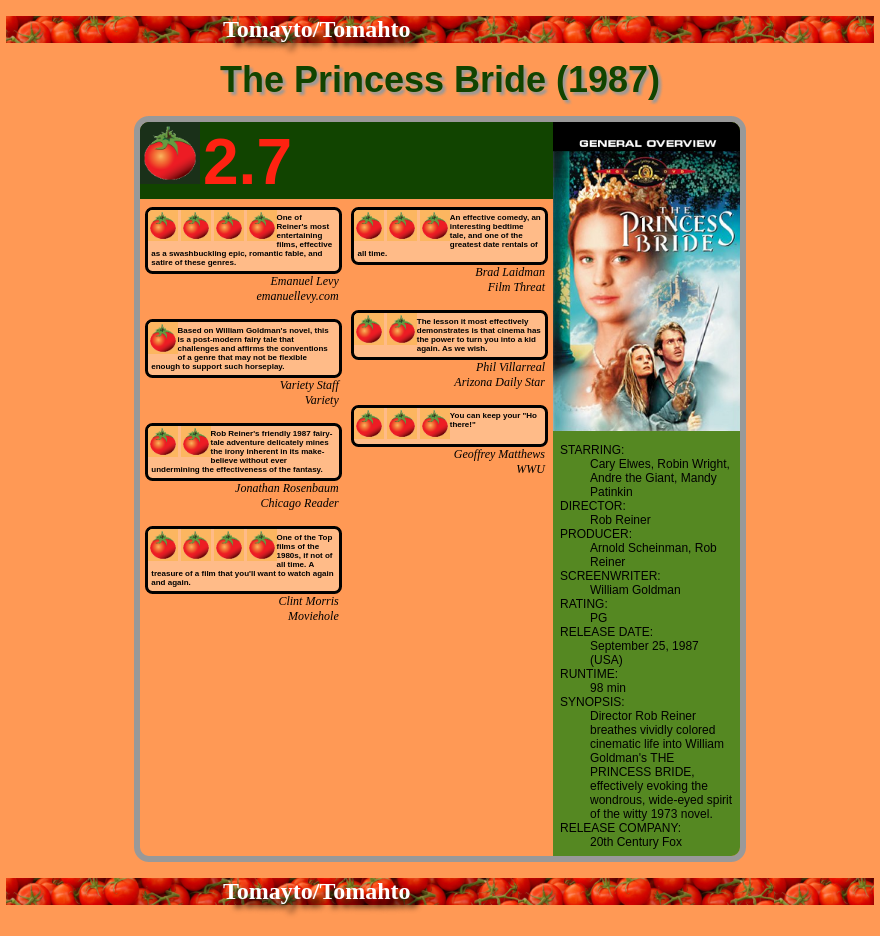
\includegraphics[width=\textwidth]{images/screenshot.png}
  \caption{Screenshot of final webpage.}
\label{screenshot}
\end{figure}

\end{document}
